In this section we will go through which design considerations we had when making the game.\\

\subsection{Game Features}
The game prototype we created has the following features:

\begin{enumerate}
	\item iOS Mobile Application
	\item Text story
	\item Events with player choice
	\item Event and character pictures with simple animations and sounds
	\item Map, where you can select where to go (Only on place to choose from in the prototype)
	\item Battle system where dogs battle eachother
	\item Ability to train dogs
	\item Ability to catch dogs (Will never succeed in the prototype)
	\item Option to breed dogs (Will never succeed in the prototype)
\end{enumerate}

\begin{figure}[h!] 
	\centering
    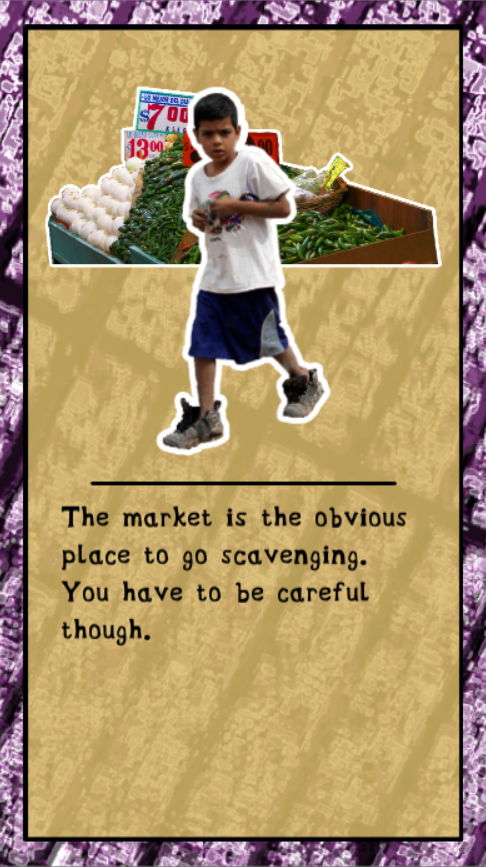
\includegraphics[width=0.5\textwidth]{GameScreen1.png}
    \caption{Story screen from the \textit{Rat Kid Dog Fight} prototype}
    \label{fig:GameScreen}
\end{figure}

%why did we choose which features?

\subsection{Covering Prototype Limitations}
While we were creating a limited and deterministic prototype, we made several considerations, to hide the procedural and deterministic nature of the prototype. These include the map system, the ability to catch and breed, which all speak to a bigger game than the prototype is. The reason for doing this was to create an illusion of a longer game, and a potentially longer relationship with the dog. We feared that if the player knew the scale of the prototype or the already determined outcomes, they would not allow themselves to become emotionally attached to the dog. \\

To create this illusion the UI is not build for simply supporting the features of the prototype, but also to support the affordances a longer and less procedural game could include. The option to 'Breed' the dogs is a feature that is not actually included in the prototype, but since the player is forced to only catch dogs of one specific gender, they will never discover this.\\

\subsection{Lack of Player Agency in Fights}
As mentioned in \ref{Agency} we have implemented impotent options in the dog fights, which aims to create the illusion of agency. These options mimic the \textit{Pokémon} games, as seen in figure \ref{fig:PokeBattle} and \ref{fig:DogFightBattle}. 

\begin{figure}[h!] 
	\centering
    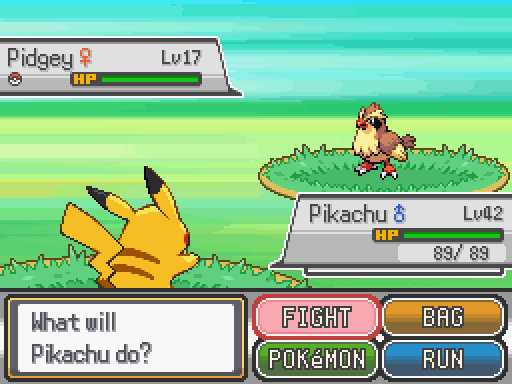
\includegraphics[width=0.5\textwidth]{PokemonBattle.png}
    \caption{A \textit{Pokémon} battle}
    \label{fig:PokeBattle}
\end{figure}

\begin{figure}[h!]
	\centering
    \includegraphics[width=0.5\textwidth]{battle.png}
    \caption{A \textit{Rat Kid Dog Fight} battle}
    \label{fig:DogFightBattle}
\end{figure}

All these battle options does not have any effect on the actual battle. The \textit{'Fight'} option let the player select between 

Impotent options. Mimicing the Pokemon games we initially implemented the following fight options ‘Fight’, ‘Use Item’, ‘Switch Dog’, ‘Run’. The options did not do anything within the game.

Goal with no player agency is to create a feeling of helplessness and hopefully the realization of no agency will put them in the place of the kid. 
\commenting{ref to 'Papers, Please'}

\subsection{Battle System}
Even though the player has limited agency in the fight system, we still simulate the fights with a very game-like system.


\commenting{insert the data behind the system}



\subsection{Actions Between Fights}
Choosing a vertical display for the phone for accessibility and to signal the briefness of the play session.

By only allowing one choice per game week, we implicitly associate a cost with the action, and an investment in your dog.
